\documentclass[compress,10pt,aspectratio=169]{beamer}
%\setbeamertemplate{background canvas}[bottom=white,top=structure.fg!25]
%\usetheme{Hannover}
%\setbeamertemplate{headline}{}
%\setbeamertemplate{footline}{}
\setbeamersize{text margin left=0.1cm}
\usepackage{appendixnumberbeamer}
\usepackage{hyperref,listings,picinpar,mathtools} % ,enumitem}
\usepackage{color}
\settowidth{\leftmargini}{\usebeamertemplate{itemize item}}
\addtolength{\leftmargini}{\labelsep}
\usepackage{fancyvrb}
%\usepackage{xcolor}
\beamertemplatenavigationsymbolsempty

\definecolor{grey}{rgb}{0.95,0.95,0.95}
\definecolor{red}{rgb}{1.0,0.0,0.0}
\definecolor{green}{rgb}{0.0,0.6,0.0}
\definecolor{blue}{rgb}{0.0,0.0,1.0}
\lstloadlanguages{bash,Java,C,C++,csh,make,sh}%%[Visual]Basic,xml}
\lstset{frame=none,basicstyle=\tiny,breaklines,tabsize=2,captionpos=b,prebreak={\hbox{$\rightarrow$}},postbreak={\hbox{$\hookrightarrow$}},showstringspaces=false,backgroundcolor=\color{grey}\bfseries,keywordstyle=\color{blue},commentstyle=\color{green}\textit,stringstyle=\color{red}\ttfamily,abovecaptionskip=2pt,aboveskip=0pt,belowskip=0pt,belowcaptionskip=0pt}
%\lstset{moredelim=[is][\color{red}]{_+_}{_+_}}

\beamertemplatefootpagenumber
% \setbeamertemplate{footline}[page number]{}
%\setbeamertemplate{page number in head/foot}{}

\setbeamertemplate{footline}[text line]{\hspace*{15.6cm}\insertpagenumber}
\setbeamertemplate{navigation symbols}{}

\usepackage{graphicx,verbatim,multicol,amsmath,bm}
\graphicspath{{./figures/}{../pictures/}}

\title{Yet Another White Rabbit running on a low-cost, generic FPGA board}
\author{\'Emilien Decoux, Jean-Michel Friedt\\ \ \\ 
FEMTO-ST Time \& Frequency department, Besan\c con, France \\ \ 
\\ \ \\ emilien.decoux@edu.univ-fcomte.fr, jmfriedt@femto-st.fr \ \\ \ \\
project archive at \url{https://github.com/oscimp/wr_acorn}\\
%\vspace{-1.27cm}
\parbox{1.0\linewidth}{
\includegraphics[width=.3\linewidth]{logo_femto.pdf}\hfill

\includegraphics[width=.27\linewidth]{WR_logo_on_white}}\vspace{-1cm}  
}

\begin{document}
\maketitle

\begin{frame}[fragile]\frametitle{Context and outline}

\vspace{0.1cm}
{\footnotesize
\begin{itemize}
\item White Rabbit (WR) supported boards require two {\bf dedicated} oscillators for generating
the digital phase detector (DMTD)
\item WR as feature of generic boards (RF signal acquisition and synthesis, {\bf Software 
Defined Radio} -- SDR) requires getting rid of this requirement
\end{itemize}
}
\begin{minipage}[t]{\linewidth}
\begin{minipage}{.55\linewidth}    
{\footnotesize
\begin{itemize}
\item $\Rightarrow$ {\bf timing library compatible with any existing FPGA based acquisition/synthesis
board} (at the expense of performance?)
\item Use of clocking circuits internal to the FPGA for generating WR clocks
\footnote{See ``More challenging that I can imagine'' on slide 8 of D. Charlet {\em \& al}, {\em Performance evaluation of a versatile and low-jitter
White Rabbit board} at 13th White Rabbit Workshop, CERN (Mar. 2024)}
\item Demonstration on Enjoy Digital's Acorn CLE215+ board...
\item ... Xilinx Artix-7 A100T FPGA / 1 Gb DDR $\Rightarrow$ start from Nikhef's  CLBv3 design and Missing Link Electronics' 2024 contribution\footnotemark
\footnotemark
\end{itemize}
}
\end{minipage}
\begin{minipage}{.49\linewidth}
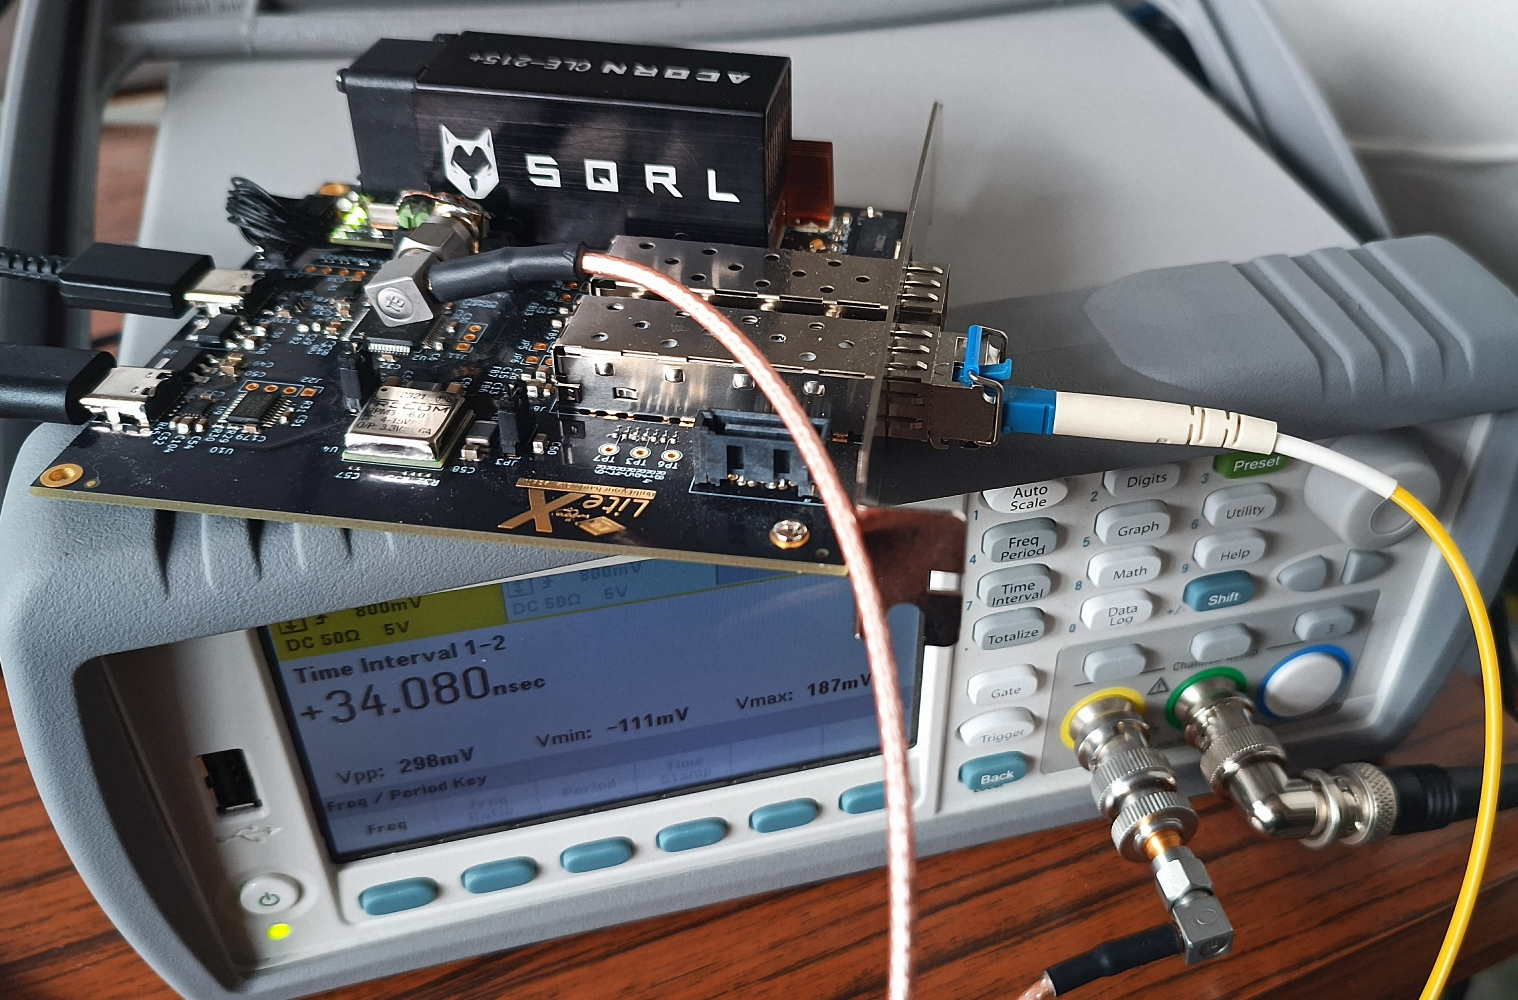
\includegraphics[width=\linewidth]{IMG_20250425_163316_728.jpg}
\end{minipage}
\end{minipage}
\footnotetext{\url{https://enjoy-digital-shop.myshopify.com/products/litex-acorn-baseboard-mini-sqrl-acorn-cle215}}
\footnotetext{13th White Rabbit Workshop (CERN), \url{https://www.missinglinkelectronics.com/wp-content/uploads/2024/03/MLE-Light-Rabbit-Presentation-at-13th-White-Rabbit-Workshop.pdf}}
\end{frame}


\begin{frame}[fragile]
\frametitle{Mixed-Mode Clock Manager (MMCM) phase-shifts for VCXO replacement}
\begin{minipage}{.74\linewidth}
Simulation v.s experimental phase noise spectra

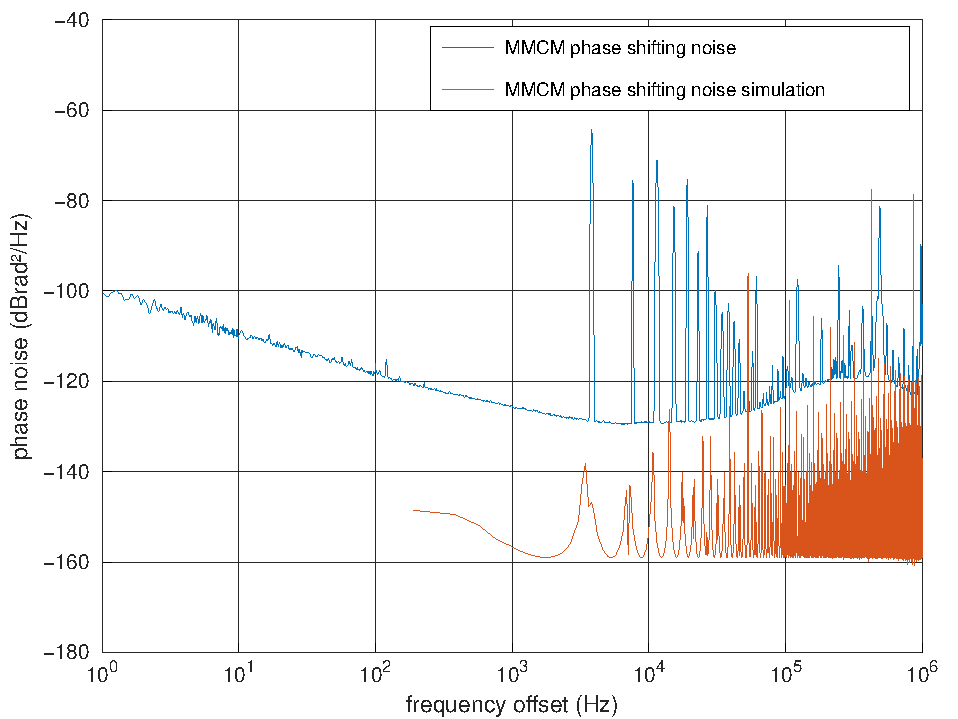
\includegraphics[width=.77\linewidth]{mmcm_phase_noise.pdf}

$\rightarrow$ accurate understanding of the MMCM spurious sources
\end{minipage}
\begin{minipage}{.25\linewidth}
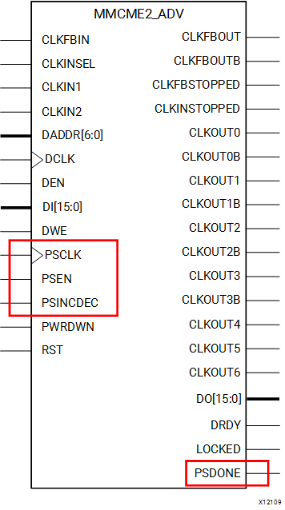
\includegraphics[width=\linewidth]{mmcm.png}
\end{minipage}
\end{frame}


\begin{frame}[fragile]\frametitle{VCO-less DMTD implementation and phase detection characterization}

What element of the control loop is limiting overall performance?

\vspace{0.3cm}
\begin{minipage}[t]{1.06\linewidth}
\begin{minipage}{.49\linewidth}

\only<1>{\input{figures/principle.pspdftex}}
\only<2>{\vspace{-0.2cm}\begin{minipage}[t]{\linewidth}
DDMTD characterization setup
\vspace{0.4cm}

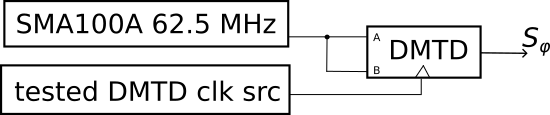
\includegraphics[width=0.9\linewidth]{dmtd_setup.png}
\vspace{0.2cm}
\end{minipage}
}

\begin{itemize}
\item Initial tests of CMOD-A7 Artix-7 generic board
\item PLL frequency $f_{PLL}=62.5$~MHz and beatnote $f_b=3$~kHz $\Rightarrow$ counter $c$ converted
to phase as $$\varphi=2\pi\cdot c\cdot f_b/f_{PLL}$$
\item phase to phase noise density $$S_\varphi=\frac{\sigma^2_\varphi}{f_b}\mbox{ @ }f_b$$
\item phase spectral density using {\tt pwelch} $\nearrow$
\end{itemize}
\end{minipage}
\begin{minipage}{.49\linewidth}
\vspace{0.6cm}
%All control loop steps characterized in the frequency domain (phase noise
%at $f_{Fourier}$ offset from carrier) and time domain (Allan deviation)

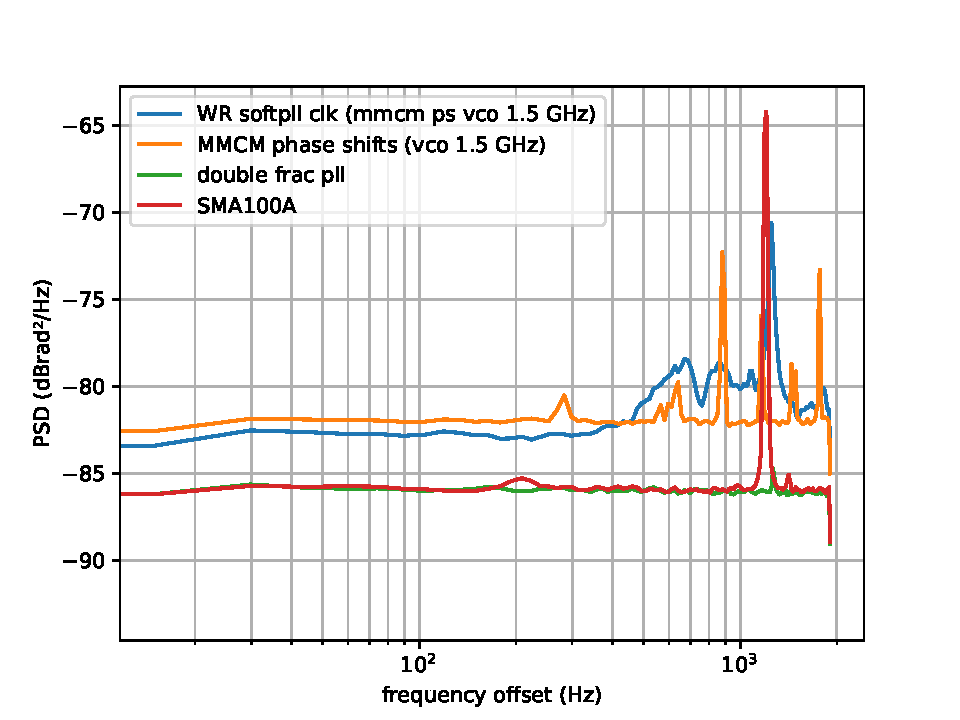
\includegraphics[width=1.05\linewidth]{dmtd_phase_noise_by_clk_src.pdf}
\end{minipage}
\end{minipage}
\end{frame}

\begin{frame}[fragile]\frametitle{Reference clock characteristics}

\begin{minipage}[t]{\linewidth}
\begin{minipage}{.49\linewidth}
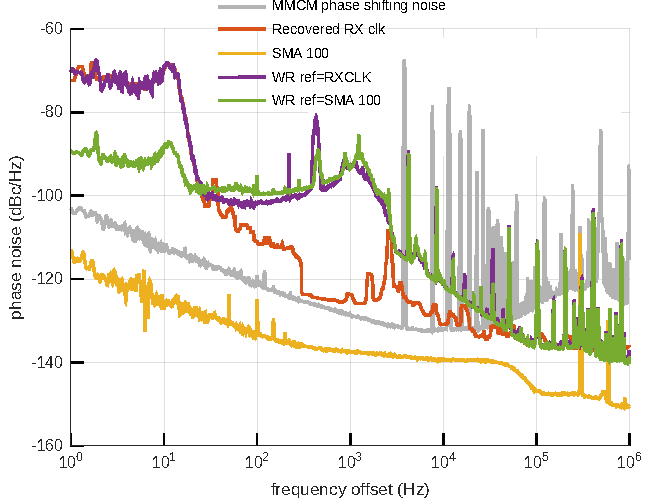
\includegraphics[width=\linewidth]{phase_noise.pdf}
\end{minipage}
\begin{minipage}{.54\linewidth}
\input{figures/principle.pspdftex}
\vspace{0.4cm}

  \begin{itemize}
    \item 1 -- 20 Hz: limited by RX clock from GTP
    \item 20 Hz -- 3.8 kHz: limited by DMTD and/or softPLL
    \item 3.8 kHz -- 1 MHz: limited by VCO (MMCM with phase-shifts)
    \item 5 kHz -- 1 MHz: spurious from MMCM with phase-shifts
  \end{itemize}
\end{minipage}
\end{minipage}
\end{frame}

\begin{frame}[fragile]\frametitle{HDL implementation on CLE215+: {\footnotesize\url{https://github.com/oscimp/wr_acorn}}}

  \begin{itemize}
    \item \texttt{board/acorn/} - FPGA-internal HDL
      \begin{itemize}
        \item \texttt{Manifest.py} - hdlmake imports
        \item \texttt{wr\_acorn\_pkg.vhd} - hdl header
        \item \texttt{xwrc\_board\_acorn.vhd} - logic around \texttt{xwrc\_platform\_xilinx} and \texttt{xwrc\_board\_common}
          \begin{itemize}
            \item \texttt{xwrc\_board\_common} expose dac interfaces outputs and clock inputs
            \item traditionnal WR convert \texttt{data+load} to I²C/other dac protocol
            \item VCO-less WR convert \texttt{data+load} to MMCM's phase-shift control
          \end{itemize}
      \end{itemize}
    \item \texttt{top/acorn\_ref\_design/} - FPGA/board interface files

          \texttt{acorn\_wr\_ref\_top.xdc} - set io pins and allow internal clocking of the GTP ports
    \item \texttt{syn/acorn\_ref\_design/} - synthesis related files
          add custom \texttt{bitstream.tcl} to allow internal clocking of the GTP ports
    \item \texttt{platform/Xilinx} - add generic to allow internal clocking of the GTP ports
  \end{itemize}

\end{frame}


\begin{frame}[fragile]\frametitle{LiteX implementation on CLE215+ \& M2SDR:\\
\vspace{-.3cm}{\footnotesize\url{https://github.com/enjoy-digital/litex_wr_nic}}}

\vspace{.3cm}
\begin{minipage}[t]{1.05\linewidth}
\begin{minipage}{.66\linewidth}
{\scriptsize
\begin{Verbatim}[commandchars=\\\{\}]
wrc# pll stat
softpll: mode:3 seq:ready n_ref 1 n_out 1
irqs:123226 alignment_state:0 {\color{green}HL1 ML1} HY=23493 MY=40133 DelCnt=0 setpoint:13037 refcnt:66565 tagcnt:53
softpll: ptracker0: enabled 1 n_avg 512 value 13575
wrc# gui
SPA7 WRPC Monitor wrpc-v5.0-ohwr-9-g5ac04dd5-dirt | Esc/q = exit; r = redraw

TAI Time: 2023-03-03-11:55:43  UTC offset: 37   PLL mode: BC  state: Locked
---+-------------------+-------------------------+---------+---------+-----
 # |        MAC        |       IP (source)       |    RX   |    TX   | VLAN
---+-------------------+-------------------------+---------+---------+-----
 0 | 22:33:44:55:66:77 |                         |     555 |     183 |    0
--- HAL ---|------------- PPSI ------------------------------------------------
 Itf | Frq |  Config   | MAC of peer port  |    PTP/EXT/PDETECT States   | Pro 
-----+-----+-----------+-------------------+-----------------------------+-----
 wr0 | Lck | auto      | 70:b3:d5:91:ea:f0 | SLAVE    /IDLE      /EXT_ON | R-W 
Pro(tocol): R-RawEth, V-VLAN, U-UDP

--------------------------- Synchronization status ----------------------------
Servo state:          White-Rabbit: {\color{green}TRACK_PHASE}

--- Timing parameters ---------------------------------------------------------
meanDelay        :              284.572 ns
delayMS          :              284.572 ns 
delayMM          :             1097.210 ns 
delayAsymmetry   :                0.000 ns
delayCoefficient :   +0.000000000000000000  fpa   0
\end{Verbatim}
}
\end{minipage}
\begin{minipage}{.33\linewidth}
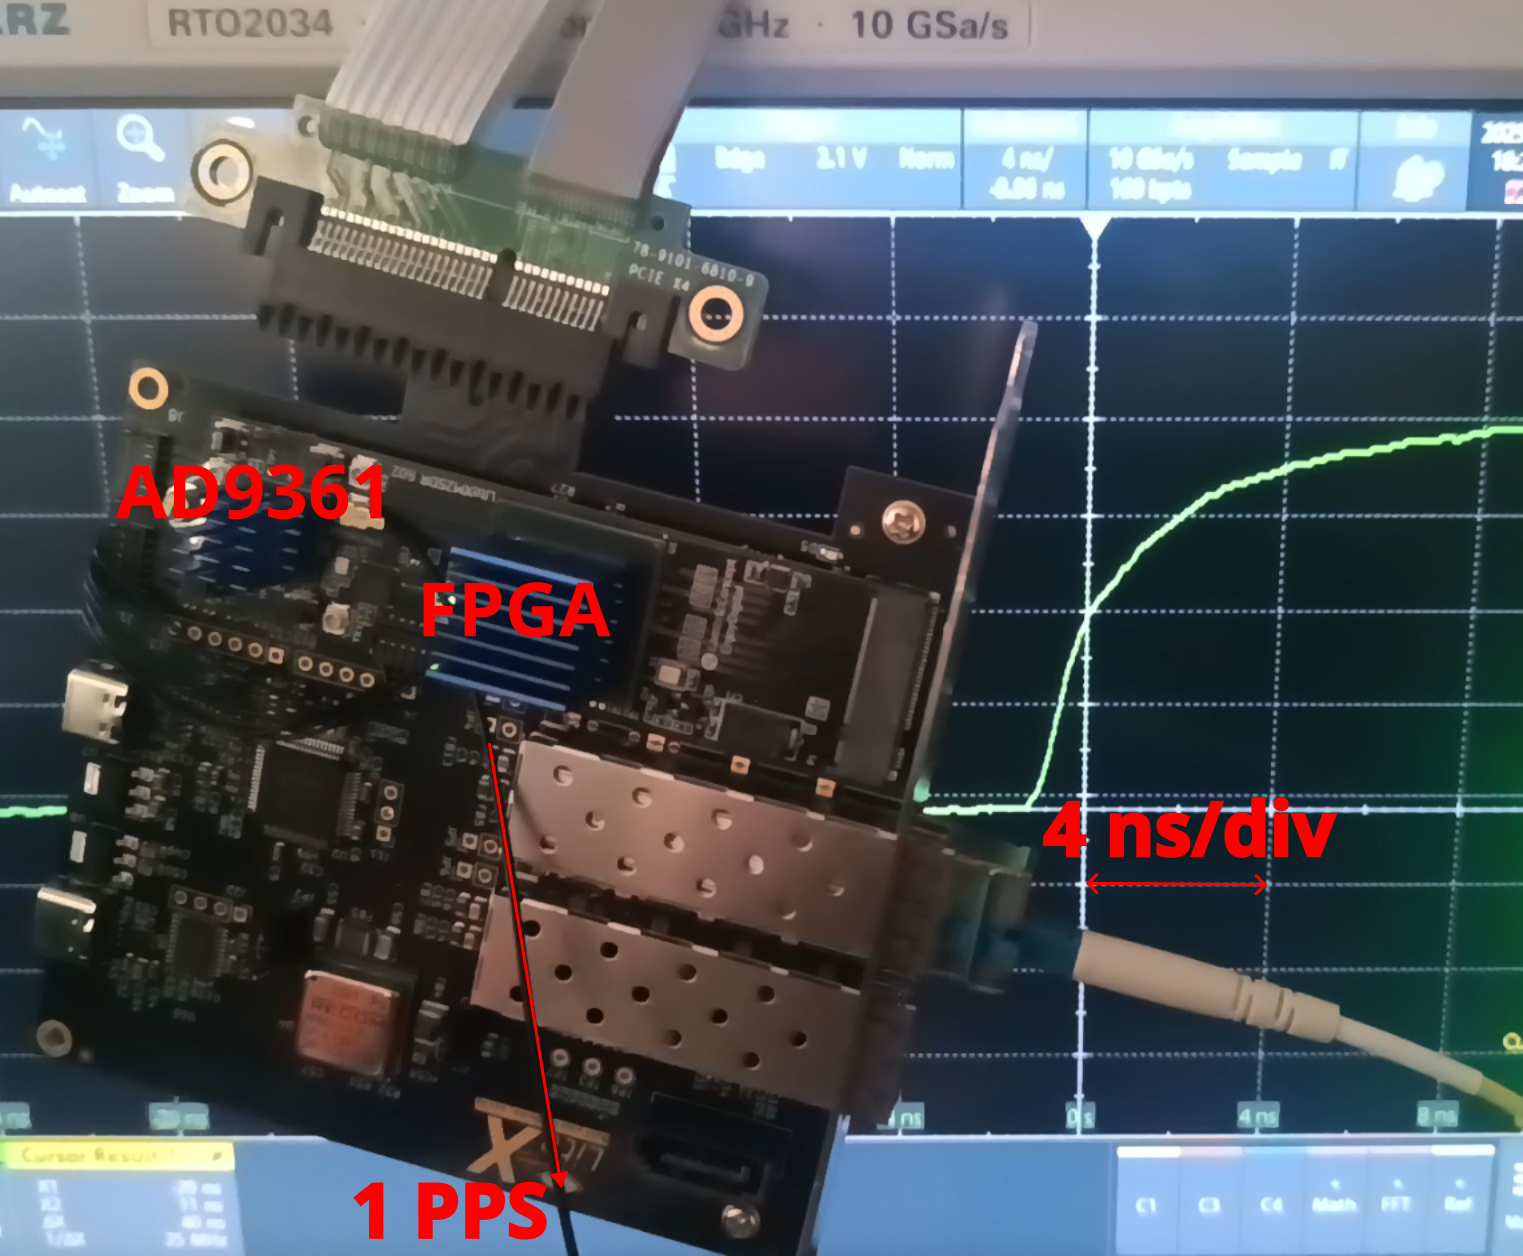
\includegraphics[width=1.06\linewidth]{figures/2025-06-16-203322_2704x1050_scrot.png}

{\footnotesize M2SDR running White-Rabbit PTP core with 1~PPS output\par}
\end{minipage}
\end{minipage}
\end{frame}

\begin{frame}[fragile]\frametitle{Results: Acorn CLE215+}

Tuning software phase locked-loop (PLL) control coefficients

\begin{minipage}[t]{1.06\linewidth}
\begin{minipage}{.49\linewidth}
\only<1>{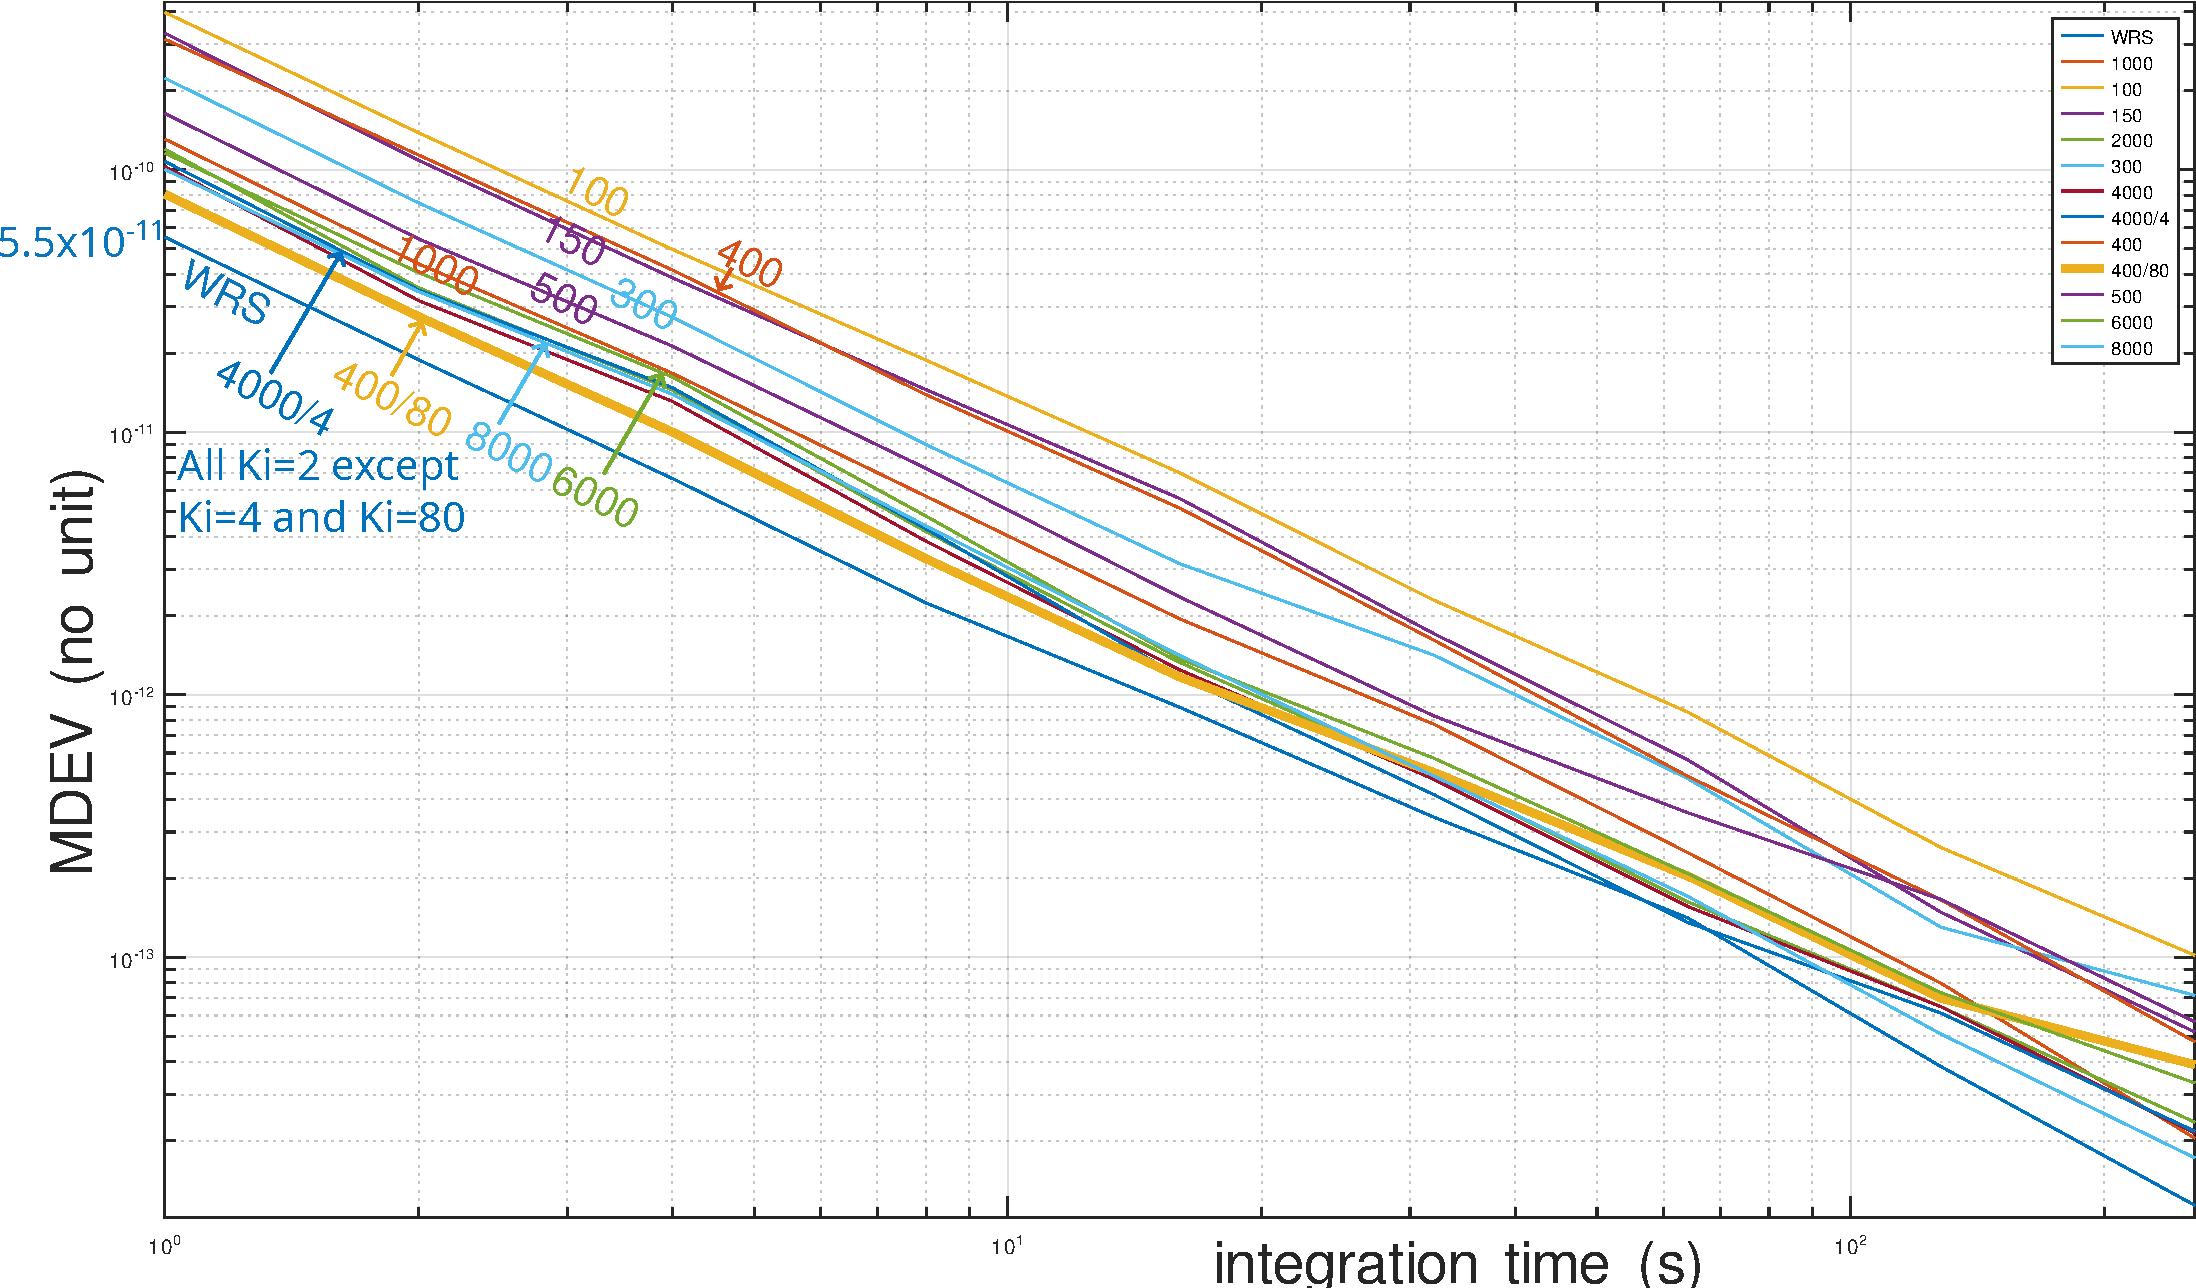
\includegraphics[width=\linewidth]{allan_wr_acorn_new.pdf}

Modified Allan deviation: phase flicker noise
}
\only<2>{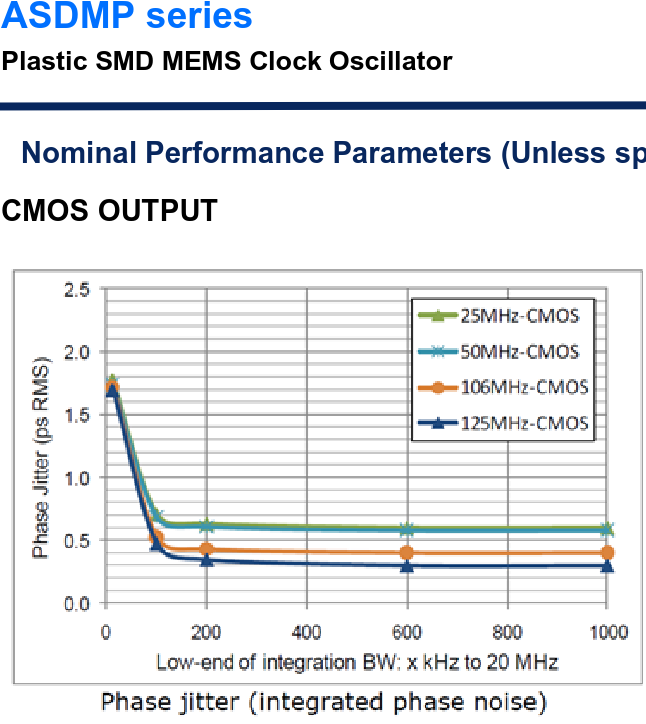
\includegraphics[width=.7\linewidth]{2025-05-30_10-12-29.png}

{\footnotesize Low quality 200~MHz MEMS oscillator (Abracon \\ASDMPLV-200.000MHZ): $\sigma_\tau=0.5$~ps @ 62.5~MHz:\\
$10\log_{10}\left(\frac{(2\pi\times 62.5\cdot 10^6\times 0.5\cdot 10^{-12})^2}{10^5}\right)=-124$~dBrad$^2$/Hz\par
\par}
}
\end{minipage}
\begin{minipage}{.49\linewidth}
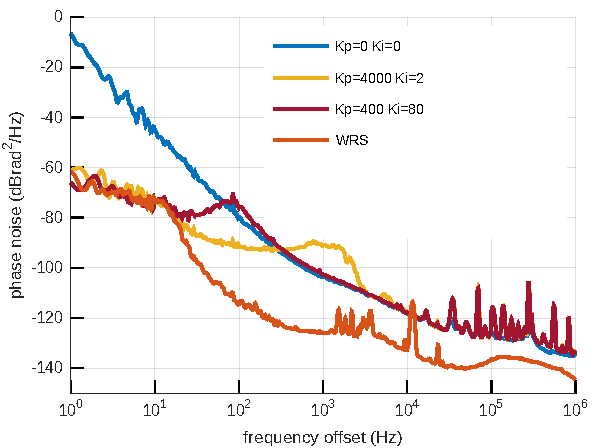
\includegraphics[width=\linewidth]{phase_noise_litex.pdf}

Phase noise (Rohde \& Schwarz FSWP, 10~MHz output)
\end{minipage}
\end{minipage}


\end{frame}

\begin{frame}[fragile]\frametitle{Results: M2SDR}

\begin{minipage}[t]{1.07\linewidth}
\begin{minipage}{.49\linewidth}
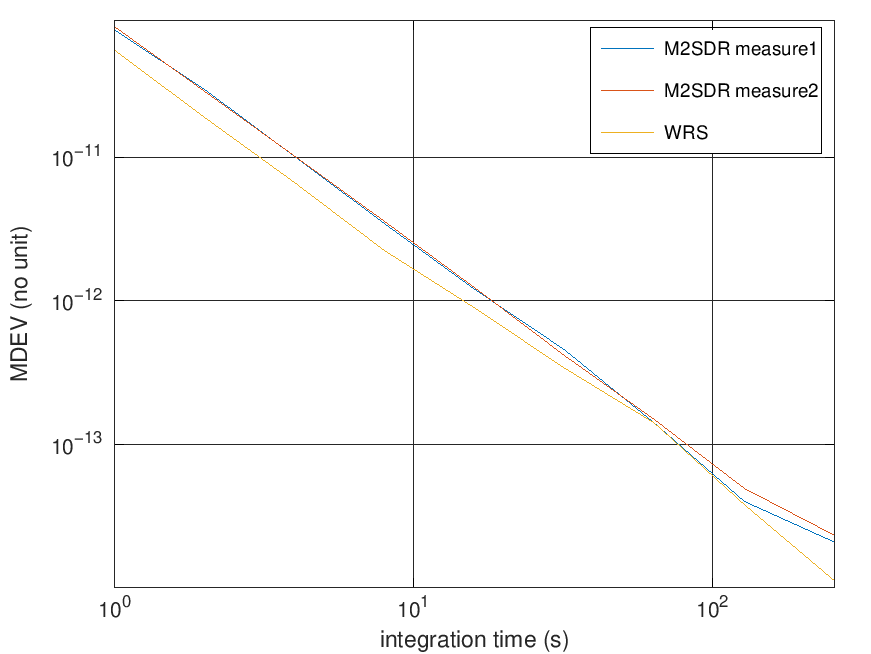
\includegraphics[width=\linewidth]{M2SDR_vs_WRS_allan}
\end{minipage}
\begin{minipage}{.49\linewidth}
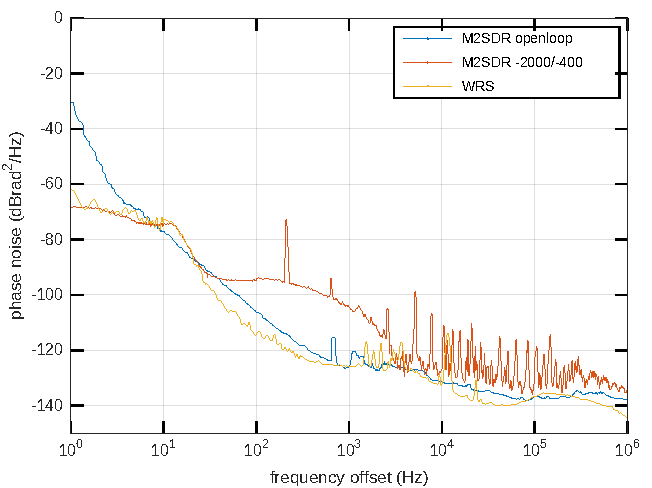
\includegraphics[width=\linewidth]{m2sdr.pdf}
\end{minipage}
\end{minipage}

100~MHz TCXO oscillator
\end{frame}

\begin{frame}[fragile]\frametitle{Conclusion \& perspectives}

\vspace{.11cm}
\begin{minipage}[t]{\linewidth}
\begin{minipage}{.55\linewidth}
{\footnotesize
\begin{itemize}
\item Initial steps for becoming familiar at FEMTO-ST with WR architecture and internals on Artix7
\item Functional demonstration, repository at \url{https://github.com/oscimp/wr_acorn}
\item Impact of internal oscillator usage on phase noise and Allan deviation performance
\item In progress: port to M2SDR {\bf with its AD9361 frontend}
\item {\bf Challenge}: can modern FPGA, with flexible clock sources, compete with high stability external (quartz)
oscillators?
\end{itemize}

\vspace{.11cm}
{\bf Acknowledgements:}
\begin{itemize}
    \item Peter Jansweijer (Nikhef) for updating the CLBv3 design, 
    \item Frederik Pfautsch (Missing Link Electronics) for committing the various VCO-less implementations, 
    \item Florent Kermarrec and Gwenhael Goavec-Merou (Enjoy Digital) for providing the
    hardware boards and LiteX implementations
    \item CERN's White Rabbit team (Tomasz Wlostowski, Tristan Gingold \& others) 
    \item Claudio Calosso (INRIM) for fruitful discussions $\nearrow$
    \end{itemize}
}
\end{minipage}
\begin{minipage}{.495\linewidth}
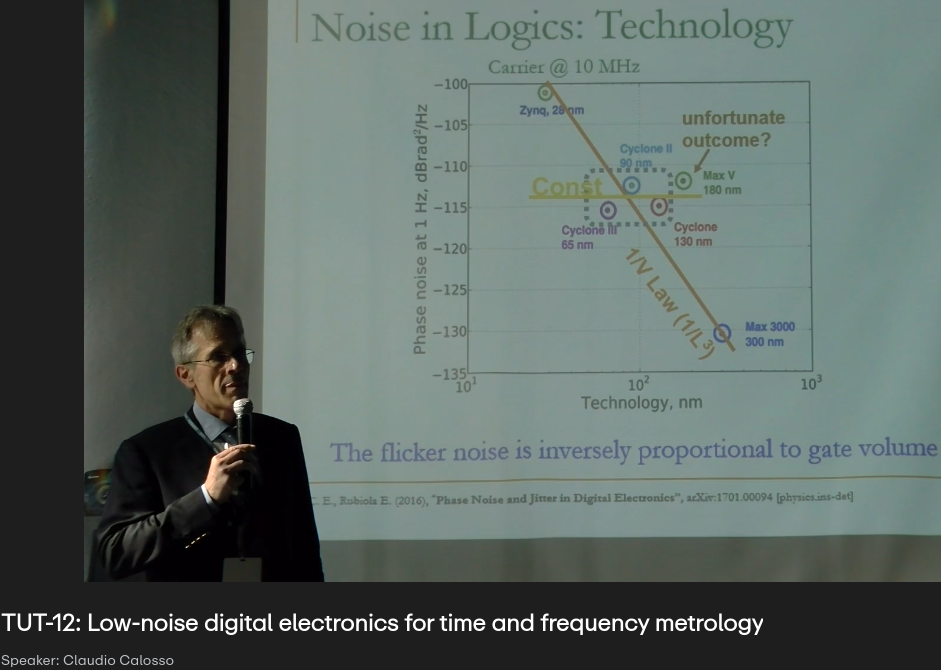
\includegraphics[width=\linewidth]{figures/2025-05-26-093826_2704x1050_scrot.png}

{\footnotesize
Impact of FPGA gate size and phase noise performance during the
2025 IFCS Tutorial on low noise digital electronics
\footnote{C.E. Calosso \& E. Rubiola {\em Phase noise and jitter in digital electronics},
Proc EFTF (2014) 374--376 at \url{https://arxiv.org/pdf/1701.00094}}\par
}
\end{minipage}
\end{minipage}
\end{frame}
\end{document}
